\documentclass[UTF8,a4paper,8pt]{ctexart} 

 \usepackage{graphicx}%学习插入图
 \usepackage{verbatim}%学习注释多行
 \usepackage{booktabs}%表格
 \usepackage{geometry}%图片
 \usepackage{amsmath} 
 \usepackage{amssymb}
 \usepackage{listings}%代码
 \usepackage{xcolor}  %颜色
 \usepackage{enumitem}%列表格式
 \usepackage{hyperref}
 \CTEXsetup[format+={\flushleft}]{section}


\geometry{left=1.6cm,right=1.8cm,top=2cm,bottom=1.7cm} %设置文章宽度

\pagestyle{plain} 		  %设置页面布局
\author{\kaishu 郑华}
\title{\heiti OpenGL4.3  学习笔记}
%代码效果定义
\definecolor{mygreen}{rgb}{0,0.6,0}
\definecolor{mygray}{rgb}{0.5,0.5,0.5}
\definecolor{mymauve}{rgb}{0.58,0,0.82}
\lstset{ %
	backgroundcolor=\color{white},   % choose the background color
	basicstyle=\footnotesize\ttfamily,        % size of fonts used for the code
	%stringstyle=\color{codepurple},
	%basicstyle=\footnotesize,
	%breakatwhitespace=false,         
	%breaklines=true,                 
	%captionpos=b,                    
	%keepspaces=true,                 
	%numbers=left,                    
	%numbersep=5pt,                  
	%showspaces=false,                
	%showstringspaces=false,
	%showtabs=false,        
	columns=fullflexible,
	breaklines=true,                 % automatic line breaking only at whitespace
	captionpos=b,                    % sets the caption-position to bottom
	tabsize=4,
	commentstyle=\color{mygreen},    % comment style
	escapeinside={\%*}{*)},          % if you want to add LaTeX within your code
	keywordstyle=\color{blue},       % keyword style
	stringstyle=\color{mymauve}\ttfamily,     % string literal style
	frame=single,					%tb top and bottom; L left double line
	xleftmargin=.06\textwidth, 
	%xrightmargin=.1\textwidth,
	rulesepcolor=\color{red!20!green!20!blue!20},
	% identifierstyle=\color{red},
	language=c++,
}

\begin{document}          %正文排版开始
 	\maketitle
 
	\newpage
	\tableofcontents
	
\newpage
\section{安装配置}
    \subsection{各种库文件}网盘环境
    
    \textbf{有时一个warnning可能就会导致全局皆输。}
    
    比如这次环境的调试程序,一个warnning4005  就是隐式转类型警告,结果就是跑不出来。最后发现是OpenGL为了兼容各系统,估计是把每个类型的字节固定了,而且还是32位,而我的是64位,导致了程序的不可运行
    
    \subsection{常见错误}
	    \subsubsection{0x70000000C}见图\ref{Glut Error},图\ref{Glut_fix}.
	    
		    解决:1- 使用glut.h , 2- 给链接输入添加\verb|glut32.lib Opengl32.lib Glu32.lib glew32.lib comctl32.lib|
		    \begin{figure}[h]
		    	\begin{center}
					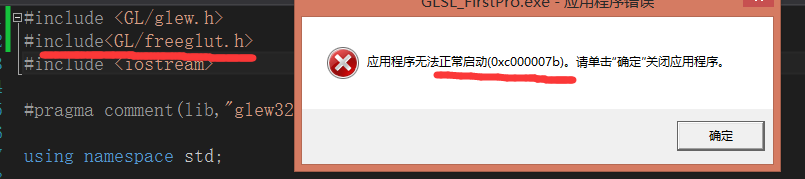
\includegraphics[scale = 0.5]{glutDoesNotMatchError.png}%就在前面括号中写图片名
		    		\caption{Error}
		    		\label{Glut Error}
		    	\end{center}
		    \end{figure}
		    \begin{figure}[h]
		    	\centering
		    	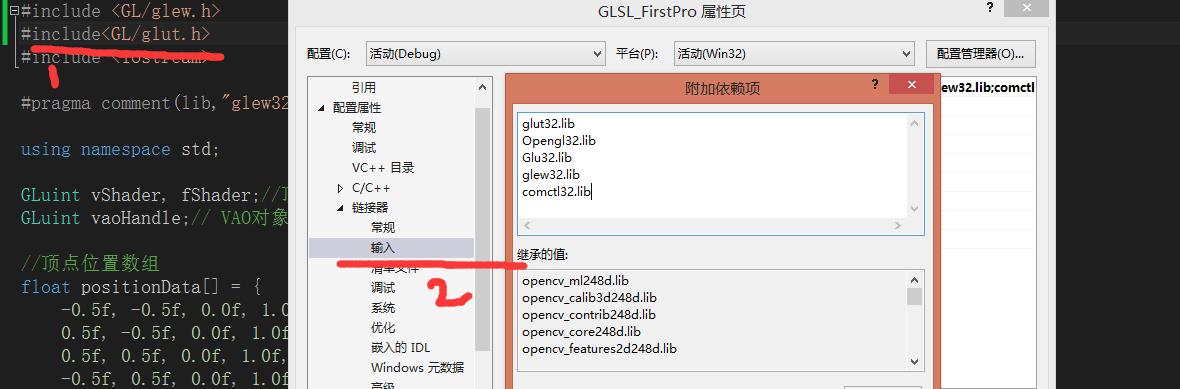
\includegraphics[scale = 0.4]{glutMatch.png}
		    	\caption{解决方法}
		    	\label{Glut_fix}
		    \end{figure}
    \subsection{参考文献} 
    \url{http://johnhany.net/2015/03/environment-for-opengl-4-with-vs2012/}    
    
\newpage
\section{四大变换}


    \subsection{参考文献} 
		 \url{http://blog.csdn.net/lyx2007825/article/details/8792475}
 
    
\newpage
\section{OpenGL基础编程}
	\subsection{渲染管线}
		\begin{figure}[h]
			\centering
			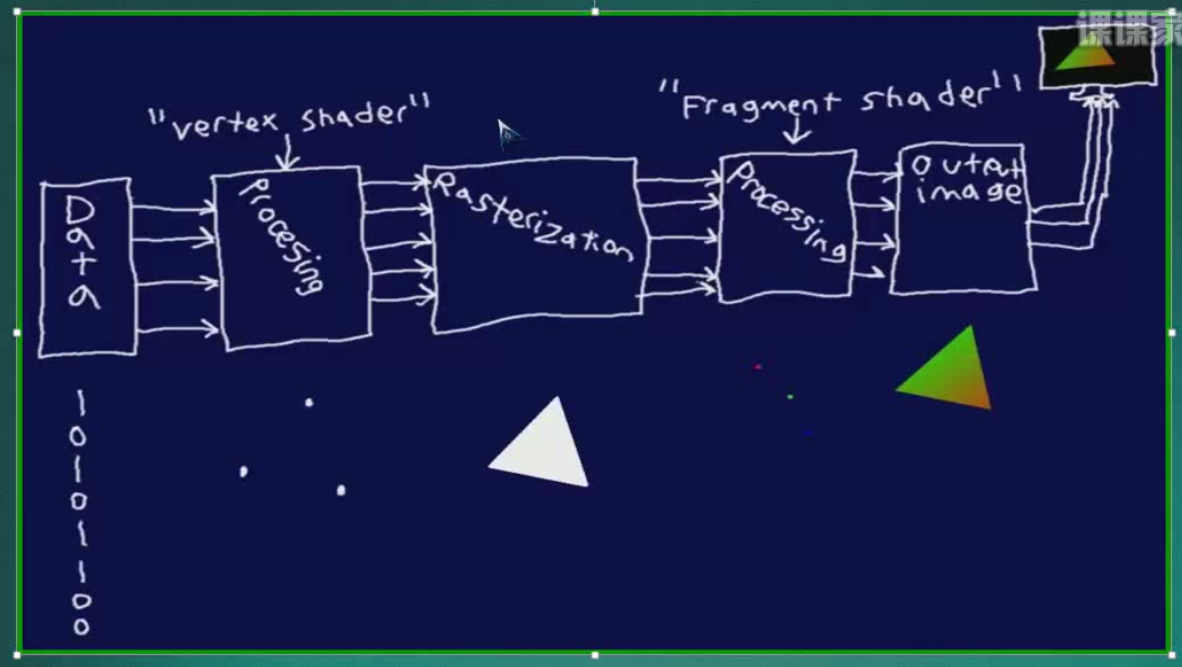
\includegraphics[scale = 0.4]{OpenGLPipeline.png}
			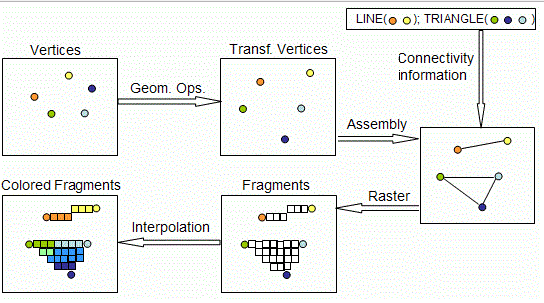
\includegraphics[scale = 0.8]{OpenGLPipeline1.png}
			\caption{OpenGL 渲染管线}
		\end{figure}

		\begin{enumerate}
			\item \textbf{数据}:顶点数据、索引数据
			\item \textbf{顶点渲染}
			\item \textbf{输出普通图形}:不渲染颜色
			\item \textbf{Fragment Shader}:顶点颜色、输出带色图形[默认白色]
		\end{enumerate}
		
		\subparagraph{参考}\url{http://blog.csdn.net/cjneo/article/details/50538033}
	\subsection{基本结构-框架}
		跟DirectX类似,都是进入消息循环然后不断监听消息。区别在于函数名可能不同,与其内部实现不同。
		有几个概念也是特别重要,其实这些就是数据准备过程和绘画过程,即Preparing to Send Data to OpenGL 和 Sending Data to OpenGL
		
		\begin{itemize}
			\item  顶点缓存对象(\textbf{Vertex Buffer Object,简称 VBO}[存在于内存中])
			\item  顶点缓存和索引缓存
			\item  缓存对象
			\item  reder()即display()
			\item 顶点数组对象 VAO (vertex array object)[显卡编程]
		\end{itemize}
		
		\subsubsection{创建顶点缓存}
			\begin{enumerate}
				\item 创建缓存对象,使用 glGenBuffers()
				\item 绑定缓存对象(指定使用哪一个缓存对象),使用 glBindBuffer()
				\item 拷贝顶点数据到缓存对象中,使用 glBufferData()
			\end{enumerate}
			
			\subparagraph{- void glGenBuffers(GLsizei n, GLuint* ids)}创建缓存对象,并返回缓存对象的标识符
				\begin{itemize}
					\item n :创建缓存对象的数量
					\item ids: 是一个 GLuint 型的变量或数组,用于储存缓存对象的单个 ID 或多个 ID
				\end{itemize}
				
			\subparagraph{- void glBindBuffer(GLenum target, GLuint id)}创建了缓存对象后,我们需要绑定缓存对象,以便使用。绑定,也就是指定当前要使用哪一个缓存对象,类似与DirectX的setStreamSource.
				\begin{itemize}
					\item target :缓存对象要存储的数据类型,只有两个值: GL\_ARRAY\_BUFFER, 和 GL\_ELEMENT\_ARRAY\_BUFFER。如果是顶点的相关属性,例如: 顶点坐标、纹理坐标、法线向量、颜色数组等,要使用 GL\_ARRAY\_BUFFER;索引数组,要使用 GL\_ELEMENT\_ARRAY\_BUFFER,以便 glDrawElements() 使用。
					
					\item id: 缓存对象的 ID
				\end{itemize}
			
			\subparagraph{- void glBufferData(GLenum target, GLsizei size, const void* data, GLenum usage)}拷贝数据到缓存对象,类似与DirectX的Lock操作.
				\begin{itemize}
					\item target: 缓存对象的类型,只有两个值: GL\_ARRAY\_BUFFER 和 GL\_ELEMENT\_ARRAY\_BUFFER
					
					\item size: 数组 data 的大小,单位是字节(bytes)
					\item data: 数组 data 的指针,如果指定为 NULL,则 VBO 只创建一个相应大小的缓存对象
					\item usage: 缓存对象如何被使用,有三中: 静态的(static)、动态的(dynamic)和流(stream).共有 9 个值:
						\begin{enumerate}
							\item GL\_STATIC\_DRAW
							\item GL\_STATIC\_READ
							\item GL\_STATIC\_COPY
							\item GL\_DYNAMIC\_DRAW
							\item GL\_DYNAMIC\_READ
							\item GL\_DYNAMIC\_COPY
							\item GL\_STREAM\_DRAW
							\item GL\_STREAM\_READ
							\item GL\_STREAM\_COPY
						\end{enumerate}
						
						\begin{itemize}
							\item Static: 指在缓存对象中的数据不能够更改(设定一次,使用很多次)
							\item Dynamic: 指数据将会频繁地更改(反复设定和使用)
							\item Stream: 指的是每一帧数据都会更改(设定一次,使用一次)
						\end{itemize}
						
						\begin{itemize}
							\item Draw: 指数据将会被送到 GPU 被用于绘制(application to GL)
							\item Read: 指数据将被读取到客户端应用程序(GL to application)
							\item Copy: 指数据将被用于绘制和读取(GL to GL)
						\end{itemize}
					\item 注意: Draw 只对 VBO 有用; Copy 和 Read 只对 PBO(像素缓存对象) 和 FBO(帧缓存对象) 有意义
				\end{itemize}
			
			\subparagraph{- void glBufferSubData(GLenum target, GLint offset, GLsizei size, void* data)}与 glBufferData() 一样,都是用于拷贝数据到缓存对象的。它能拷贝一段数据到一个已经存在的缓存,偏移量为 offset
			
			\subparagraph{- void glDeleteBuffers(GLsizei n, const GLuint* ids)}删除一个或多个缓存对象。
		
		
		\subsubsection{顶点缓存和索引缓存的使用}
			\subparagraph{1.准备顶点数据与索引数据}概念如同DirectX的绘制
				\begin{lstlisting}
	//顶点数据
	GLfloat vertexs[] = { 0.0f, 0.0f, 0.0f, 0.2f, 0.0f, 0.0f,
	-0.2f, 0.0f, 0.0f, 0.0f, 0.2f, 0.0f,
	0.0f, -0.2f, 0.0f, 0.0f, 0.0f, 0.2f,
	0.0f, 0.0f, -0.2f};
	
	//索引数据
	GLubyte indexs[] = {0,1,2,3,4,5,6};				
				\end{lstlisting}
			
			\subparagraph{2.生成缓存[数据,索引]对象,并拷贝数据}示例
				\begin{lstlisting}
	GLuint vboVertexId;
	GLuint vboIndexId;
	
	//生成数据缓存对象
	glGenBuffers(1, &vboVertexId);
	glBindBuffer(GL_ARRAY_BUFFER, vboVertexId);
	glBufferData(GL_ARRAY_BUFFER, sizeof(vertexs), vertexs, GL_STATIC_DRAW);
	
	//生成索引缓存对象
	glGenBuffers(1, &vboIndexId);
	glBindBuffer(GL_ELEMENT_ARRAY_BUFFER, vboIndexId);
	glBufferData(GL_ELEMENT_ARRAY_BUFFER, sizeof(indexs), indexs, GL_STATIC_DRAW);				
				\end{lstlisting}
				
			\subparagraph{3.使用}示例
				\begin{lstlisting}
	glEnableClientState(GL_VERTEX_ARRAY);
	glEnableClientState(GL_INDEX_ARRAY);
	
	glBindBuffer(GL_ARRAY_BUFFER, vboVertexId);
	glVertexPointer(3, GL_FLOAT, 0, 0);
	
	glBindBuffer(GL_ELEMENT_ARRAY_BUFFER, vboIndexId);
	glIndexPointer(GL_UNSIGNED_BYTE, 0, 0);
	
	//... 绘制图形
	
	glDisableClientState(GL_VERTEX_ARRAY); 
	glDisableClientState(GL_INDEX_ARRAY);
	glBindBuffer(GL_ARRAY_BUFFER, 0);				
				\end{lstlisting}
				
			\subparagraph{4.利用顶点绘图方法}示例
				\begin{lstlisting}
	//1. 第一种
	glBegin(GL_POINTS);
		glArrayElement(0);
		glArrayElement(1);
		glArrayElement(2);
		glArrayElement(5);
	glEnd();
	
	//2. 第二种  类似于DirectX的DrawPrimitive()函数
	glDrawElements(GL_POINTS, 7, GL_UNSIGNED_BYTE, 0);
	
	//3. 第三种
	glDrawArrays(GL_POINTS,0,7);				
				\end{lstlisting}
			
			\subparagraph{5.将不同类型的数据拷贝到一个缓存对象}缓存的一种用法,用 glBufferSubData() 可以将几个数据拷贝到一个缓存对象中
				\begin{lstlisting}
	GLfloat vertexs[] = {0.0f, 0.0f, 0.0f, 0.2f, 0.0f, 0.0f,
						-0.2f, 0.0f, 0.0f, 0.0f, 0.2f, 0.0f,
						0.0f, -0.2f, 0.0f, 0.0f, 0.0f, 0.2f,
						0.0f, 0.0f, -0.2f};
	
	GLfloat colors[] = {1.0f, 0.0f, 0.0f, 0.0f, 1.0f, 0.0f,
						0.0f, 0.0f, 1.0f, 1.0f, 1.0f, 0.0f,
						0.0f, 1.0f, 1.0f, 1.0f, 0.0f, 1.0f,
						0.0f, 0.0f, 0.0f};
	
	
	//现在,要将两个数组存在同一个缓存对象中,顶点数组在前,颜色数组在后
	glGenBuffers(1, &vboVertexId);
	glBindBuffer(GL_ARRAY_BUFFER, vboVertexId);
	glBufferData(GL_ARRAY_BUFFER, sizeof(vertexs)+sizeof(colors), 0, GL_STATIC_DRAW);
	glBufferSubData(GL_ARRAY_BUFFER, 0, sizeof(vertexs) , vertexs);    //注意第三个参数,偏移量
	glBufferSubData(GL_ARRAY_BUFFER, sizeof(vertexs), sizeof(colors), colors);
	
	
	//创建好缓存对象后,要用 glVertexPointer 和 glColorPointer 指定相应的指针位置。
	//但是,由于 glColorPointer 的最后一个参数,必须是指针类型。
	
	//glColorPointer 的最后一个参数用偏移量指示了颜色数组的位置
	glEnableClientState(GL_VERTEX_ARRAY);
	glEnableClientState(GL_COLOR_ARRAY);
	glEnableClientState(GL_INDEX_ARRAY);
	
	glBindBuffer(GL_ARRAY_BUFFER, vboVertexId);
	glVertexPointer(3, GL_FLOAT, 0, 0);
	glColorPointer(3,GL_FLOAT,0,(void*)sizeof(vertexs));    //注意最后一个参数
	
	glBindBuffer(GL_ELEMENT_ARRAY_BUFFER, vboIndexId);
	glIndexPointer(GL_UNSIGNED_BYTE, 0, 0);
	
	glDrawArrays(GL_POINTS,0,7);
	
	glDisableClientState(GL_VERTEX_ARRAY); 
	glDisableClientState(GL_COLOR_ARRAY); 
	glDisableClientState(GL_INDEX_ARRAY);
	glBindBuffer(GL_ARRAY_BUFFER, 0);				
				\end{lstlisting}
			
			\subparagraph{6.缓存对象的实时修改}在DirectX这个东西没搞出来,这竟然有个方法。
				比起显示列表,VBO 一个很大的优点是能够读取和修改缓存对象的数据。最简单的方法是重新拷贝虽有数据到 VBO,利用 glBufferData() 和 glBufferSubData(),这种情况下,你的程序必须要保存有两份数据:一份在客户端(CPU),一份在设备端(GPU)
				
				另一种方法,是\textbf{将缓存对象映射到客户端,再通过指针修改数据}
				
				 \textbf{- void* glMapBuffer(GLenum target, GLenum access)}
				 
					 映射当前绑定的缓存对象到客户端,glMapBuffer 返回一个指针,指向缓存对象。如果 OpenGL 不支持,则返回 NULL
				
					如果 OpenGL 正在操作缓存对象,此函数不会成功,直到 OpenGL 处理完毕为止。为了避免等待,可以先用 glBindBuffer(GL\_ARRAY\_BUFFER, 0) 停止缓存对象的应用,再调用 glMapBuffer
					
					\begin{itemize}
						\item target:GL\_ARRAY\_BUFFER 或 GL\_ELEMENT\_ARRAY\_BUFFER
						\item access:值有三个 GL\_READ\_ONLY、 GL\_WRITE\_ONLY、 GL\_READ\_WRITE,分别表示只读、只写、可读可写
					\end{itemize}
					
				\textbf{- GLboolean glUnmapBuffer(GLenum target)}
				
					修改完数据后,将数据反映射到设备端
					
				\begin{lstlisting}
	glBindBuffer(GL_ARRAY_BUFFER, vboVertexId);
	GLfloat* ptr = (float*)glMapBuffer(GL_ARRAY_BUFFER, GL_WRITE_ONLY);
	
	if(ptr)
	{
		ptr[0] = 0.2f;  ptr[1] = 0.2f;  ptr[2] = 0.2f;
		glUnmapBuffer(GL_ARRAY_BUFFER);
	}
	
	glBindBuffer(GL_ARRAY_BUFFER, 0);				
				\end{lstlisting}
		\subsubsection{顶点缓存和顶点数组的使用:VAO、VBO}
			\subparagraph{VAO}是这样一种方式:\textbf{把对象信息直接存储在图形卡中},\textit{而不是在当我们需要的时候传输到图形卡}。这就是Direct3D所采用得方式,而在OpenGL中只有OpenGL3.X以上的版本中采用。这就意味着我们的应用程序不用将数据传输到图形卡或者是从图形卡输出,这样也就获得了额外的性能提升.
			
			\subparagraph{使用}使用VAO并不难。我们不需要大量的glVertex调用,而是把顶点数据存储在数组中,然后放进VBO,最后在VAO中存储相关的状态。记住:VAO中并没有存储顶点的相关属性数据。OpenGL会在后台为我们完成其他的功能。
				\begin{enumerate}[itemindent = 1em]
					\item \textbf{产生VAO}:\textit{void glGenVertexArrays(GLsizei n,GLuint *arrays);}
						\begin{itemize}
							\item n:要产生的VAO对象的数量
							\item arrays:存放产生的VAO对象的名称
						\end{itemize}
						
					\item \textbf{绑定VAO}: \textit{void glBindVertexArray(GLuint array)};
						\begin{itemize}
							\item arrays:要绑定的顶点数组的名字
						\end{itemize}
						
					\item \textbf{产生VBOs}: \textit{void glGenBuffers(GLsizei   n,GLuint *   buffers)};参考上
					\item \textbf{绑定VBOs}:\textit{void glBindBuffer(GLenum   target,GLuint   buffer)};
					
					\item \textbf{给VBO分配数据}:\textit{void glBufferData( GLenum target,GLsizeiptr size,const GLvoid *  data,GLenum   usage)};
						\begin{itemize}
							\item target可能取值为:
								\begin{itemize}
									\item GL\_ARRAY\_BUFFER(表示顶点数据)
									\item GL\_ELEMENT\_ARRAY\_BUFFER(表示索引数据)	
									\item GL\_PIXEL\_PACK\_BUFFER(表示从OpenGL获取的的像素数据)
									\item GL\_PIXEL\_UNPACK\_BUFFER(表示传递给OpenGL的像素数据)
								\end{itemize}
							\item size:缓冲区对象字节数
							\item data:指针:指向用于拷贝到缓冲区对象的数据。或者是NULL,表示暂时不分配数据
						\end{itemize}
					\item \textbf{定义存放顶点属性数据的数组,启用VAO中对应的顶点属性数组},\textit{void glEnableVertexAttribArray( GLuint  index)}
					
					\item \textbf{给对应的顶点属性数组指定数据}:\textit{void glVertexAttribPointer(GLuint  index,GLint size,GLenum  type,GLboolean  normalized,GLsizei  stride,const GLvoid*  pointer)};
					
					\item \textbf{然后在进行渲染的时候,只需要绑定对应的VAO即可}:\textit{glBindVertexArray(vaoHandle)};
					
					\item \textbf{使用完毕之后需要清除绑定}:\textit{glBindVertexArray(0)};
				\end{enumerate}
		\subsubsection{使用VAO Mesh 类示例}
			\subparagraph{VAO[直接使用图形卡缓存绘图]-代码}示例如下:
			\begin{lstlisting}
	// 顶点
	class Vertex{
	public:
		Vertex(const glm::vec3& pos):this->pos = pos{}
	private:
		glm::vec3 pos;
	};
	
	// 网格
	class Mesh{
	public:
		Mesh(Vertex* vertices, unsigned int numVertices)
		{
			m_drawCount = numVertices;
			
			glGenVertexArrays(1, &m_vertexArrayObject);
			glBindVertexArray(m_vertexArrayObject);
			
			glGenBuffers(NUM_BUFFERS, m_vertexArrayBuffers);
			glBindBuffer(GL_ARRAY_BUFFER, m_vertexArrayBuffer[POSITION_VB]);
			glBufferData(GL_ARRAY_BUFFER, numVertices * sizeof(vertices[0]), vertices, GL_STATIC_DRAW);
			
			glEnableVertexAttribArray(0);
			glVertexAttribPointer(0,3, GL_FLOAT, GL_FALSE, 0, 0);
			
			glBindVertexArray(0);
		}
		~Mesh()
		{
			glDeleteVertexArrays(1, &m_vertexArrayObject);
		}
		
		void Draw()
		{
			glBindVertexArray(m_vertexArrayObject);
			
			glDrawArrays(GL_TRIANGLES, 0, m_drawCount);// 第三个参数为总共的 顶点个数,当然画三角形s,就是3的倍数咯
			
			glBindVertexArray(0);
		}
	private:
		enum{
			POSTION_VB,
			NUM_BUFFERS
		};
		GLuint m_vertexArrayObject;
		GLuint m_vertexArrayBuffer[NUM_BUFFERS];
		usigned int m_drawCount;
	};
	
	// Main 调用Mesh Draw
		Vertex vertices[] = {Vertex(glm::vec3(-0.5,-0.5,0)),
							 Vertex(glm::vec3(0,0.5,0)),
							 Vertex(glm::vec3(0.5,-0.5,0)),}
							 
		Mesh mesh(vertices, sizeof(vertices)/sizeof(vertices[0]));
			\end{lstlisting}
			
		\subparagraph{结果}
			实现结果见图\ref{VAOResult}:
			\begin{figure}[h]
				\centering
				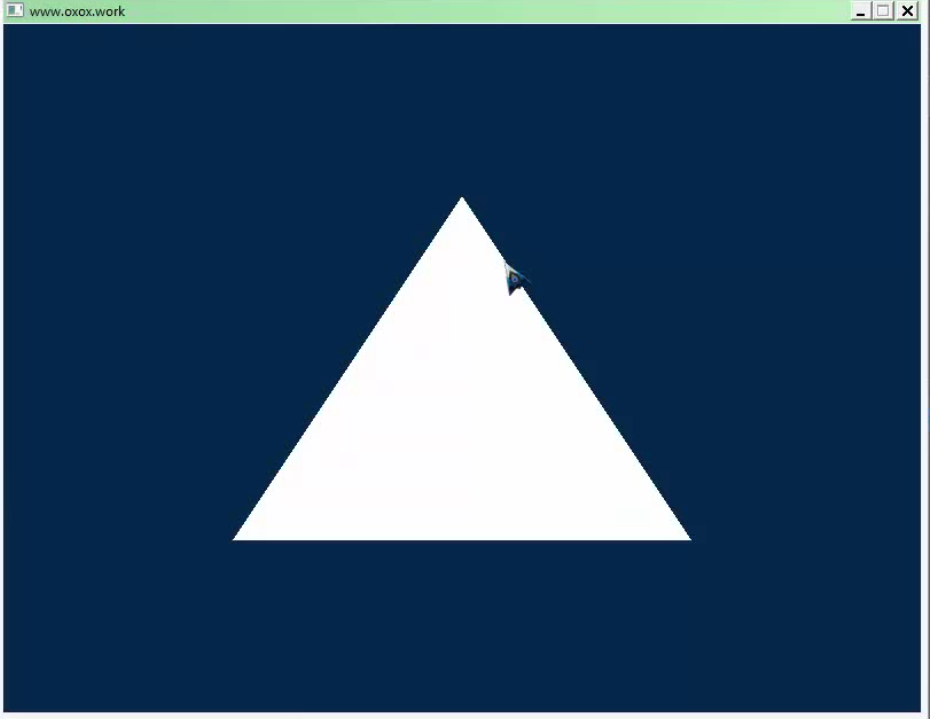
\includegraphics[scale = 0.5]{VBOMeshResult.png}
				\caption{上述Mesh代码绘画效果}
				\label{VAOResult}
			\end{figure}
	
	\subsection{光照添加}
	
	\subsection{纹理添加}
			
	\subsection{着色器-GLSL}
		OpenGL着色语言(OpenGL Shading Language,GLSL)是用来在OpenGL中着色编程的语言,是一种具有C/C++风格的高级过程语言,同样也以main函数开始,只不过执行过程是在GPU上。GLSL使用类型限定符而不是通过读取和写入操作来管理输入和输出。着色器主要分为顶点着色器(Vertex Shader)和片段着色器(Fragment Shader)两部分
		\subsubsection{顶点着色器}
			\subparagraph{主要功能}
				\begin{itemize}[itemindent = 1em]
					\item 顶点法线变换及单位化
					\item 纹理坐标变换
					\item 光照参数生成
				\end{itemize}
			\subparagraph{输入内容}
				\begin{itemize}[itemindent = 1em]
					\item 着色器源代码
					\item attribute变量
					\item uniform变量
				\end{itemize}
			\subparagraph{输出内容}
				\begin{itemize}[itemindent = 1em]
					\item varying变量
					\item 内置的特殊变量,如\verb|gl_Position、gl_FrontFacing、gl_PointSize|
				\end{itemize}
		\subsubsection{片段着色器}
			\subparagraph{主要功能}
				\begin{itemize}[itemindent = 1em]
					\item 在差值得到的值上进行操作
					\item 访问纹理
					\item 应用纹理
					\item 雾化
					\item 颜色融合
				\end{itemize}
			\subparagraph{输入内容}
				\begin{itemize}[itemindent = 1em]
					\item 着色器源代码
					\item 用户自定义的varying变量
					\item uniform变量
					\item 采样器(Sampler)
					\item 一些内置的特殊变量(\verb|gl_PointCoord、gl_FragCoord、gl_FrontFacing等)|	
				\end{itemize}
			\subparagraph{输出内容}:内置的特殊变量\verb|gl_FragColor|
		\subsubsection{程序组成}
			在OpenGL程序中\textbf{使用着色器}一般需要依次执行以下步骤:
				\begin{enumerate}[itemindent = 1em]
					\item 顶点着色程序的源代码和片段着色程序的源代码分别写入到一个文件里(或字符数组)里面,一般顶点着色器源码文件后缀为\textbf{.vert},片段着色器源码文件后缀为\textbf{.frag}
					\item \textbf{使用glCreateshader()}分别创建一个顶点着色器对象和一个片段着色器对象
					\item \textbf{使用glShaderSource()}分别将顶点/片段着色程序的源代码字符数组绑定到顶点/片段着色器对象上
					\item \textbf{使用glCompileShader()}分别编译顶点着色器和片段着色器对象(最好检查一下编译的成功与否)
					\item \textbf{使用glCreaterProgram()}创建一个着色程序对象
					\item \textbf{使用glAttachShader()}将顶点和片段着色器对象附件到需要着色的程序对象上
					\item \textbf{使用glLinkProgram()}分别将顶点和片段着色器和着色程序执行链接生成一个可执行程序(最好检查一下链接的成功与否)
					\item \textbf{使用glUseProgram()}将OpenGL渲染管道切换到着色器模式,并使用当前的着色器进行渲染
				\end{enumerate}	
				\subparagraph{示例}
					以下是一个功能简单但流程完整的使用顶点着色器和片段着色器渲染的矩形图形。项目一共包含5个文件。2个资源文件(VertexShader.vert和FragmentShader.frag,分别是顶点着色器源码文件和片段着色器源码文件),2个cpp文件(Hello GLSL.cpp和Textfile.cpp),1个头文件Textfile.h。
					
					\textbf{整体流程}如下所示:
						\begin{figure}[h]
							\centering
							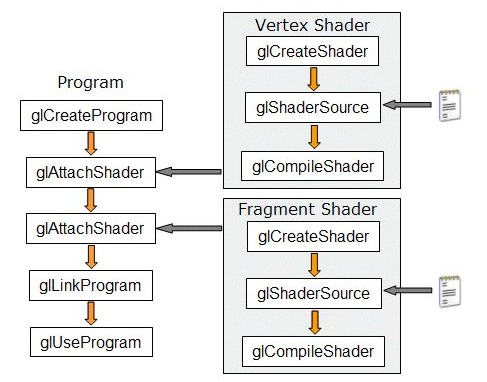
\includegraphics[width = 12cm, height = 6cm]{GLSLProcess.png}
							\caption{GLSL 流程}
							\label{GLSL}
						\end{figure}
					
					\begin{itemize}[itemindent = 1em]
						\item 准备\textbf{原始顶点数据}
							\begin{lstlisting}
	GLuint vaoHandle;// VAO对象  
	
	//顶点位置数组    
	float positionData[] = {-0.5f,-0.5f,0.0f,1.0f,  
							0.5f,-0.5f,0.0f,1.0f,  
							0.5f,0.5f,0.0f,1.0f,  
							-0.5f,0.5f,0.0f,1.0f};  
	//顶点颜色数组    
	float colorData[] = {1.0f, 0.0f, 0.0f,1.0f,  
					 	 0.0f, 1.0f, 0.0f,1.0f,  
						 0.0f, 0.0f, 1.0f,1.0f,  
						 1.0f,1.0f,0.0f,1.0f};  						
	
	void initVBO()  
	{  
		//绑定VAO  
		glGenVertexArrays(1, &vaoHandle);  
		glBindVertexArray(vaoHandle);  
		
		// Create and populate the buffer objects    
		GLuint vboHandles[2];  
		glGenBuffers(2, vboHandles);  
		GLuint positionBufferHandle = vboHandles[0];  
		GLuint colorBufferHandle = vboHandles[1];  
		
		//绑定VBO以供使用    
		glBindBuffer(GL_ARRAY_BUFFER, positionBufferHandle);  
		//加载数据到VBO    
		glBufferData(GL_ARRAY_BUFFER, 16 * sizeof(float),  
		positionData, GL_STATIC_DRAW);  
		
		//绑定VBO以供使用    
		glBindBuffer(GL_ARRAY_BUFFER, colorBufferHandle);  
		//加载数据到VBO    
		glBufferData(GL_ARRAY_BUFFER, 16 * sizeof(float),  
		colorData, GL_STATIC_DRAW);  
		
		glEnableVertexAttribArray(0);//顶点坐标    
		glEnableVertexAttribArray(1);//顶点颜色    
		
		//调用glVertexAttribPointer之前需要进行绑定操作    
		glBindBuffer(GL_ARRAY_BUFFER, positionBufferHandle);  
		glVertexAttribPointer(0, 4, GL_FLOAT, GL_FALSE, 0, (GLubyte *)NULL);  
		glBindBuffer(GL_ARRAY_BUFFER, colorBufferHandle);  
		glVertexAttribPointer(1, 4, GL_FLOAT, GL_FALSE, 0, (GLubyte *)NULL);  
	}  
							\end{lstlisting}
						\item 准备\textbf{着色器代码}
							\begin{lstlisting}
	// 顶点着色器:VertexShader.vert 
	//定义GLSL版本    
	#version 430    
	
	in vec4 VertexPosition;    
	in vec4 VertexColor;  
	
	out vec4 Color;    
	
	void main()    
	{    
		Color =VertexColor;    
		gl_Position = VertexPosition;  
	}    
	
	// 片段着色器:FragmentShader.frag
	#version 440       
	in vec4 Color;   //汉字用于测试汉字是否可用,有报着色器源码注释含汉字运行报错的  
	
	out vec4 FragColor;      
	
	void main()    
	{    
		FragColor = Color;    
	}    
							\end{lstlisting}
						\item \textbf{创建着色器对象}
							\begin{lstlisting}
							
	// 读取着色器代码文件-将其转换为字符穿传入GLSL 编译器
	// 读入字符流  
	char *textFileRead(const char *fn)  
	{  
		FILE *fp;  
		char *content = NULL;  
		int count = 0;  
		if (fn != NULL)  
		{  
			fp = fopen(fn, "rt");  
			if (fp != NULL)  
			{  
				fseek(fp, 0, SEEK_END);  
				count = ftell(fp);  
				rewind(fp);  
				if (count > 0)  
				{  
					content = (char *)malloc(sizeof(char) * (count + 1));  
					count = fread(content, sizeof(char), count, fp);  
					content[count] = '\0';  
				}  
				fclose(fp);  
			}  
		}  
		return content;  
	}  
					
							
	GLuint vShader, fShader;//顶点/片段着色器对象 
	void initShader(const char *VShaderFile, const char *FShaderFile)  
	{  
		// 1、查看显卡、GLSL和OpenGL的信息    
		const GLubyte *vendor = glGetString(GL_VENDOR);  
		const GLubyte *renderer = glGetString(GL_RENDERER);  
		const GLubyte *version = glGetString(GL_VERSION);  
		const GLubyte *glslVersion = glGetString(GL_SHADING_LANGUAGE_VERSION);  
		cout << "显卡供应商   : " << vendor << endl;  
		cout << "显卡型号     : " << renderer << endl;  
		cout << "OpenGL版本   : " << version << endl;  
		cout << "GLSL版本     : " << glslVersion << endl;  
		
		// 2、编译着色器    
		//创建着色器对象:顶点着色器    
		vShader = glCreateShader(GL_VERTEX_SHADER);  
		//错误检测    
		if (0 == vShader)  
		{  
			cerr << "ERROR : Create vertex shader failed" << endl;  
			exit(1);  
		}  
		
		//把着色器源代码和着色器对象相关联    
		const GLchar *vShaderCode = textFileRead(VShaderFile);  
		const GLchar *vCodeArray[1] = { vShaderCode };  
		
		//将字符数组绑定到对应的着色器对象上  
		glShaderSource(vShader, 1, vCodeArray, NULL);  
		
		//编译着色器对象    
		glCompileShader(vShader);  
		
		//检查编译是否成功    
		GLint compileResult;  
		glGetShaderiv(vShader, GL_COMPILE_STATUS, &compileResult);  
		if (GL_FALSE == compileResult)  
		{  
			GLint logLen;  
			//得到编译日志长度    
			glGetShaderiv(vShader, GL_INFO_LOG_LENGTH, &logLen);  
			if (logLen > 0)  
			{  
				char *log = (char *)malloc(logLen);  
				GLsizei written;  
				//得到日志信息并输出    
				glGetShaderInfoLog(vShader, logLen, &written, log);  
				cerr << "vertex shader compile log : " << endl;  
				cerr << log << endl;  
				free(log);//释放空间    
			}  
		}  
		
		//创建着色器对象:片断着色器    
		fShader = glCreateShader(GL_FRAGMENT_SHADER);  
		//错误检测    
		if (0 == fShader)  
		{  
			cerr << "ERROR : Create fragment shader failed" << endl;  
			exit(1);  
		}  
		
		//把着色器源代码和着色器对象相关联    
		const GLchar *fShaderCode = textFileRead(FShaderFile);  
		const GLchar *fCodeArray[1] = { fShaderCode };  
		glShaderSource(fShader, 1, fCodeArray, NULL);  
		
		//编译着色器对象    
		glCompileShader(fShader);  
		
		//检查编译是否成功    
		glGetShaderiv(fShader, GL_COMPILE_STATUS, &compileResult);  
		if (GL_FALSE == compileResult)  
		{  
			GLint logLen;  
			//得到编译日志长度    
			glGetShaderiv(fShader, GL_INFO_LOG_LENGTH, &logLen);  
			if (logLen > 0)  
			{  
				char *log = (char *)malloc(logLen);  
				GLsizei written;  
				//得到日志信息并输出    
				glGetShaderInfoLog(fShader, logLen, &written, log);  
				cerr << "fragment shader compile log : " << endl;  
				cerr << log << endl;  
				free(log);//释放空间    
			}  
		}  
		
		//3、链接着色器对象    
		//创建着色器程序    
		GLuint programHandle = glCreateProgram();  
		if (!programHandle)  
		{  
			cerr << "ERROR : create program failed" << endl;  
			exit(1);  
		}  
		//将着色器程序链接到所创建的程序中    
		glAttachShader(programHandle, vShader);  
		glAttachShader(programHandle, fShader);  
		//将这些对象链接成一个可执行程序    
		glLinkProgram(programHandle);  
		//查询链接的结果    
		GLint linkStatus;  
		glGetProgramiv(programHandle, GL_LINK_STATUS, &linkStatus);  
		if (GL_FALSE == linkStatus)  
		{  
			cerr << "ERROR : link shader program failed" << endl;  
			GLint logLen;  
			glGetProgramiv(programHandle, GL_INFO_LOG_LENGTH,  
			&logLen);  
			if (logLen > 0)  
			{  
				char *log = (char *)malloc(logLen);  
				GLsizei written;  
				glGetProgramInfoLog(programHandle, logLen,  
				&written, log);  
				cerr << "Program log : " << endl;  
				cerr << log << endl;  
			}  
		}  
		else//链接成功,在OpenGL管线中使用渲染程序    
		{  
			glUseProgram(programHandle);  
		}  
	}  
							\end{lstlisting}
						\item \textbf{使用着色器}渲染
							\begin{lstlisting}
	void init()  
	{  
		//初始化glew扩展库    
		GLenum err = glewInit();  
		if (GLEW_OK != err)  
		{  
			cout << "Error initializing GLEW: " << glewGetErrorString(err) << endl;  
		}  
		//加载顶点和片段着色器对象并链接到一个程序对象上  
		initShader("VertexShader.vert","FragmentShader.frag");  
		//绑定并加载VAO,VBO  
		initVBO();  
		glClearColor(0.0, 0.0, 0.0, 0.0);  
	}  
	
	// 显示函数
	void display()  
	{  
		glClear(GL_COLOR_BUFFER_BIT);  
		//使用VAO、VBO绘制    
		glBindVertexArray(vaoHandle);  
		glDrawArrays(GL_TRIANGLE_FAN, 0, 4);  
		glBindVertexArray(0);  
		glutSwapBuffers();  
	} 
	
	// 键盘监听 ESC键用于退出使用着色器  
	void keyboard(unsigned char key, int x, int y)  
	{  
		switch (key)  
		{  
		case 27:  
			glDeleteShader(vShader);  
			glUseProgram(0);  
			glutPostRedisplay(); //刷新显示  
			break;  
		}  
	}   
	
	// Main
	int main(int argc, char** argv)  
	{  
		glutInit(&argc, argv);  
		glutInitDisplayMode(GLUT_DOUBLE | GLUT_RGB);  
		glutInitWindowSize(600, 600);  
		glutInitWindowPosition(100, 100);  
		glutCreateWindow("Hello GLSL"); 
		 
		init();  
		glutDisplayFunc(display);  
		glutKeyboardFunc(keyboard); 
		 
		glutMainLoop();  
		return 0;  
	}  
							\end{lstlisting}
					\end{itemize}
					
		\subsubsection{参考文献}
			着色器:\url{http://blog.csdn.net/dcrmg/article/details/53648306}
\newpage			
\section{MFC with OpenGL}
	\subsection{环境配置}
		\url{http://blog.csdn.net/sircarfield/article/details/6992586}
		
		\url{http://www.cnblogs.com/phinecos/archive/2007/07/28/834916.html}
		
	\subsection{闪烁解决办法}
		\url{http://blog.sina.com.cn/s/blog_6d4b374e010141ix.html}
		    
		\url{http://bbs.csdn.net/topics/390804673}
			
	\subsection{定时器概念与程序}
		\url{http://blog.sina.com.cn/s/blog_678e97f80100thp7.html}
			
			
	\subsection{坐标确定}
		左下角为原点
		
	\subsection{画椭球}
		\url{http://www.tuicool.com/articles/zmE3Mr}
		
\newpage
\section{OpenGL 读取 OBJ 文件}
    \subsection{参考文献} 
		\subparagraph{OBJ 文件格式}\url{http://guanser.blog.163.com/blog/static/2112467872012877161702/}
	
	
\newpage 
\section{OpenGL 实现天空盒子}
	\subsection{实现}
		
	\subsection{错误记录}
		\paragraph{1.error LNK1281}error LNK1281: 无法生成 SAFESEH 映像VS2013常见编译错误解决
		
		\subparagraph{解决方案}:
		
		打开项目属性的链接器的命令行,在那里输入: /SAFESEH:NO点击确定再次编译,成功解决问题

\newpage
\section{PCL  安装}
	\subsection{错误记录}
		\paragraph{1.error LNK2019} 要么是 依赖库没配置好, 要么就是32位与64位不兼容(这里包括 库与系统不兼容,还包括库与系统兼容但与编译器不兼容)
		
		如当使用 64位的库时,也是64位的系统,虽然你使用的编译器也是64位,但是在编译的时候并没有选择 x64,而选择了win32 也会出现这个错误
		
		参考该文章的更改编译器部分\url{http://www.ithao123.cn/content-8701571.html}
\end{document} 
 		    